\section{Claims, Reproducibility and Limitations}
\label{sec:record-b}

This section completes the project record begun in Section~\ref{sec:record}: the status of every claim the
repository tracks, how the evidence behind the preceding sections is kept reproducible, and what remains open.


% --------------------------------------------------------------------------------------------
\subsection{Claim Ledger}
\label{sec:record-claims}

Since 2026-10-20 every candidate statement the manuscript might make has been entered in a claim ledger
(\texttt{docs/\allowbreak{}research/\allowbreak{}CLAIMS.md}, last updated 2026-11-12), tied to a model version and an evidence source,
together with the interpretation that the evidence permits. The ledger is binding on this report: we use its
``Permitted interpretation'' column and do not upgrade any entry. Two rules shape it. First, model versions are
never merged into one study (v1--v4 of the moving-support benchmark and the separate recovery v1 are reported
separately). Second, negative and null results are retained rather than dropped: a later model version does not
erase earlier observations, an alternative method that lost (C11) is reported so that the comparison is not
selectively presented, and claims the team expected to hold but which failed (C06, C08, C25, C26) are among
the most informative results of the project. Figure~\ref{fig:record-claims} summarises the 28 entries and
Table~\ref{tab:record-ledger} transcribes them.

\begin{figure}[t]
  \centering
  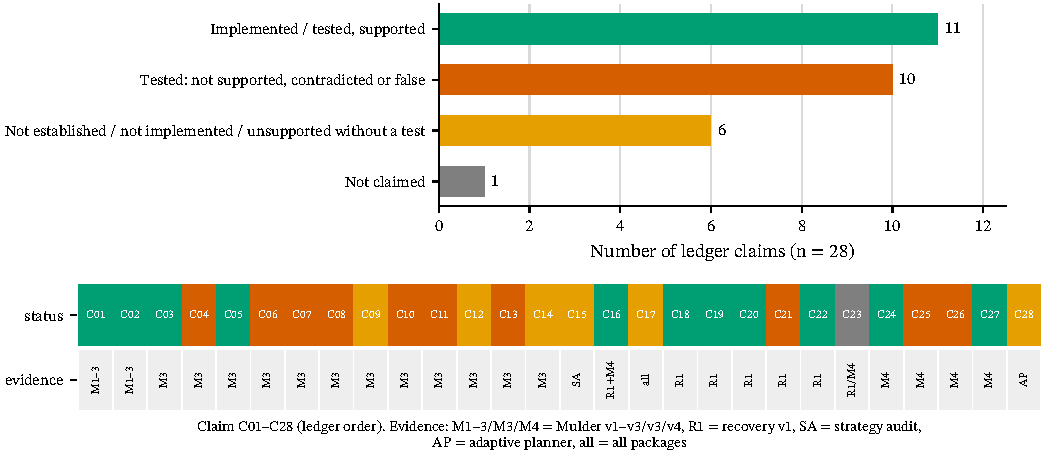
\includegraphics[width=\linewidth]{figures/record/record_claims}
  \caption{Claim-ledger summary, $n=28$ claims. \emph{Top:} claims per status category. Categories are assigned
  from the wording of the ledger's ``Status and evidence'' column: \textbf{S} supported (``Implemented'',
  ``Tested'', ``Implemented/tested''); \textbf{N} tested and negative (``Not supported'', ``Not demonstrated'',
  ``Contradicted'', ``False'', or ``Unsupported'' where the row cites a counter-result: C04, C21);
  \textbf{U} not established (``Not established'', ``Not implemented/validated'', or ``Unsupported'' because
  the relevant outputs are imposed: C09); \textbf{X} ``Not claimed''. \emph{Bottom:} each claim coloured by
  category, with the study the ledger row names as its evidence. Data:
  \texttt{docs/\allowbreak{}research/\allowbreak{}CLAIMS.md}; script \texttt{scripts/\allowbreak{}record/\allowbreak{}make\_\allowbreak{}figures.py}.}
  \label{fig:record-claims}
\end{figure}

{\footnotesize
\setlength{\tabcolsep}{3pt}
\renewcommand{\arraystretch}{1.12}
\begin{longtable}{@{}p{0.045\linewidth}p{0.22\linewidth}p{0.27\linewidth}p{0.36\linewidth}c@{}}
\caption{The claim ledger C01--C28, transcribed from \texttt{docs/\allowbreak{}research/\allowbreak{}CLAIMS.md} at \texttt{61d18d8}
(wording unchanged apart from \LaTeX{} escaping). ``Cat.'' is our category from
Figure~\ref{fig:record-claims}.}
\label{tab:record-ledger}\\
\toprule
ID & Candidate statement & Status and evidence & Permitted interpretation & Cat. \\
\midrule
\endfirsthead
\toprule
ID & Candidate statement & Status and evidence & Permitted interpretation & Cat. \\
\midrule
\endhead
\midrule
\multicolumn{5}{r}{\emph{continued}}\\
\endfoot
\bottomrule
\endlastfoot
C01 & A moving-support construction benchmark with six policies is implemented & Implemented,
  \texttt{spider\_\allowbreak{}web\_\allowbreak{}mulder}; v1--v3 & Software/domain contribution, not identified spider cognition & S \\
C02 & Endpoint-only execution is fragile in the tested moving conditions & Tested, v1/v2 and v3 endpoint profile;
  0/30 at 10\,cm and 0.05\,Hz in v3 & Failure of that executor and model, not physical impossibility or failure of
  HTN generally & S \\
C03 & Ideal continuous local feedback preserves completion in the primary moving comparison & Tested, v3 tracking
  local 30/30; Wilson 95\% approximately 0.8865--1 & Result over initial phases under assumed no-slip advection
  and ideal sensing & S \\
C04 & Moving and stationary construction have identical time & Unsupported & Local duration increases about
  0.98\%; the model's interval excludes zero. Do not claim replication of the paper's non-significant test & N \\
C05 & Moving supports cause small simulated cost changes under ideal tracking & Tested, v3; see curated paired
  intervals & Describe effect sizes/uncertainty and assumptions; no biological equivalence claim & S \\
C06 & HTN hierarchy improves disturbance tolerance over the flat baseline & Not supported, v3 flat local
  duration/outcomes match HTN on tested phases & Preserve this negative result; supplied sequence and feedback
  suffice in this benchmark & N \\
C07 & Predictive repair outperforms simple local feedback & Not demonstrated, v3 primary outcomes equal &
  Monitoring/planning costs and stress conditions must be considered & N \\
C08 & More frequent full replanning improves performance & Not supported in the primary ideal-tracking comparison
  & Full replanning adds delay and planning work without improving completion & N \\
C09 & Geometry invariance validates Mulder's biological findings & Unsupported & Counts/targets and ideal
  corrected geometry are substantially imposed; area reconstruction is an estimate & U \\
C10 & Results are robust to substantial sensory lag & Contradicted in tested profiles, 0/12 completion at 1\,s
  and 5\,s lag & Ideal sensing is an important limitation; these lag values are assumptions, not measured spider
  latencies & N \\
C11 & The \texttt{phase\_wait} alternative improves construction cost & Not supported in tested profile; slower by
  22.703291\,s on matched local moving runs & Retain alternative-method negative result, not selective reporting & N \\
C12 & The simulator is quantitatively calibrated against the original cohort & Not established; raw observations
  absent & Import/rigid-only fitting code is implemented, but availability is not a completed fit & U \\
C13 & Mulder v3 execution recovery resumes a retained HTN solution tree & False for that implementation; recovery
  v1 is separate & Describe v3 as fresh component/root re-decomposition with completed-index guards & N \\
C14 & Mulder v3 component repair handles arbitrary dependent suffixes and physical roadblocks & Not
  implemented/validated in v3 & Recovery v1 adds scoped graph/dependency cases; it does not retroactively change
  v3 & U \\
C15 & Historical Mulder runs guarantee full search backtracking among methods & Not established; installed default
  probe shows greedy commitment & New recovery baselines pin strategy; do not retroactively relabel historical runs
  & U \\
C16 & IPyHOP is a relevant backend for dependency-changing recovery & Implemented/tested in recovery v1 and opt-in
  Mulder v4; historical v3 outputs preserved & Existing prior work; custom actor integration is not a new general
  recovery algorithm & S \\
C17 & All repository packages support one joint quantitative conclusion & Not established & FAP, A*, original and
  updated HTN evidence need separate audit before synthesis & U \\
C18 & Retained-tree recovery handles the declared changed-anchor and dependent-suffix cases & Tested, recovery v1
  with pinned upstream IPyHOP; see \texttt{recovery\_\allowbreak{}v1\_\allowbreak{}summary.json} & Scoped to the shared authored sector domain
  and event protocol & S \\
C19 & New recovery performs graph-valid detours and can retrace from the observed position & Tested, recovery
  route/position assertions & Scaffold connectivity is an explicit initial condition; not arbitrary biological
  roadblock handling & S \\
C20 & Damaged completed effects are distinguished from history and restored without resource rollback & Tested,
  \texttt{prefix\_damage} and silk conservation & Requires the implemented observer and repair methods; IPyHOP does
  not infer physical damage unaided & S \\
C21 & Re-entrancy always improves planning cost & Unsupported; some infeasible cases incur more method calls &
  Report same-engine paired contrasts, including failed planning attempts & N \\
C22 & Search backtracking is explicit in the new fresh-planning baseline & Implemented,
  \texttt{iterative\_\allowbreak{}dfs\_\allowbreak{}backtracking} and strategy-restoration test & Does not change the unpinned historical
  Mulder runs & S \\
C23 & The full published Run-Lazy-Refineahead evaluation has been reproduced & Not claimed & We use actual IPyHOP
  re-entry with a custom immediate-precondition actor and a different domain & X \\
C24 & Actual Mulder HTN supports retained-tree IPyHOP recovery & Implemented/tested v4, 2,160 trials and 176 tests
  & Same geometry/executor; new segment-refinement tasks; legacy default preserved & S \\
C25 & Retained IPyHOP improves physical outcomes over fresh IPyHOP in Mulder & Not supported: all 720 pairs have
  identical completion, repairs, time and travel & Scoped to the declared direct-method profiles and two
  construction sizes & N \\
C26 & Fewer method calls mean faster retained planning in Mulder & Contradicted in primary full/filtered
  comparisons & Full saves 1.67\% method calls but increases measured planning wall time; adapters/instrumentation
  included & N \\
C27 & Lagged filtered completion can improve with whole-suffix refresh & Tested, configured-size 0/10 legacy versus
  5/10 each IPyHOP mode and GTPyhop root control & Ten diagnostic root-control trials match IPyHOP physical
  outcomes; gain is not unique to re-entrancy; small-size case regresses 3/10 to 2/10 & S \\
C28 & Restored adaptive-planner perturbation CSV demonstrates an HTN advantage & Not established; historical CSV
  and code were recovered from a local stash without a contemporaneous provenance manifest & Treat as historical,
  unaudited output; a one-seed CLI smoke check is software verification, not a scientific comparison & U \\
\end{longtable}
}

In numbers: 11 claims are supported as implemented or tested, 10 were tested and came out negative,
contradicted or false, 6 are not established, and 1 is explicitly not claimed. Of the 11 supported entries,
four describe implementations (C01, C16, C22, C24) and the rest are tested results, each scoped by its
permitted interpretation; C27 in particular is supported only together with its control, which shows the gain
is due to whole-suffix refresh rather than re-entrancy. Every candidate statement asserting an advantage for the
hierarchy, frequent replanning, predictive repair or re-entrancy (C06--C08, C21, C25, C26) came out negative.

% --------------------------------------------------------------------------------------------
\subsection{Reproducibility and Research-Record Practice}
\label{sec:record-repro}

\paragraph{The written record.}
\texttt{RESEARCH\_\allowbreak{}RECORD\_\allowbreak{}GUIDELINES.md} and \texttt{AGENTS.md} make the record part of every substantive
change: append the change, rationale, validation and output locations to the work log; update the claim ledger
when evidence supports, weakens or limits a claim, distinguishing implemented, tested and proposed mechanisms;
record exact settings, seeds, simulator and planner versions, search strategy and source hashes; preserve
historical output directories; keep curated evidence and figures under \texttt{docs/}; and separate software
verification, computational experiments and empirical biological validation. The index
(\texttt{docs/\allowbreak{}research/\allowbreak{}README.md}) lists each record and states its scope: the four packages that predate the
Mulder branch ``have not all been independently audited or experimentally validated''. Manuscript-ready prose
for the Mulder, recovery and v4 studies lives in \texttt{docs/\allowbreak{}manuscript/\allowbreak{}}, and \texttt{.ai-memory/} holds a
short project memory and roadmap that point back to these files.

\paragraph{Curated evidence with input hashes.}
Each completed study has a curated JSON in \texttt{docs/\allowbreak{}research/\allowbreak{}evidence/\allowbreak{}}, produced by a snapshot script in
\texttt{docs/\allowbreak{}research/\allowbreak{}probes/\allowbreak{}}, which stores the selected results together with the SHA-256 of its input files,
the hashes of the executed source, the runtime versions (Python 3.12.0, GTPyhop 1.9.7, NetworkX 3.4.2,
NumPy 2.2.6), the seeds and the uncertainty method (paired bootstrap, 2,000 replicates, RNG seed 20261020;
the unit of uncertainty is the initial forcing phase, ``not biological individual''). Figure reuse is tracked in
\texttt{docs/\allowbreak{}manuscript/\allowbreak{}figures/\allowbreak{}provenance.json}, which maps every curated figure to its source file and hash.

\paragraph{Snapshots and committed results.}
On 2026-10-27 all 3,046 generated files under \texttt{mulder\_results/} were archived as
\texttt{research\_\allowbreak{}snapshots/\allowbreak{}mulder\_\allowbreak{}results\_\allowbreak{}2026-10-27.tar.gz} (19,120,445 bytes) with a manifest of per-file
SHA-256 hashes and restoration instructions. On 2026-11-12 the same files were committed under
\texttt{mulder\_results/} (commit \texttt{d2e639b}), although the directory is otherwise ignored by Git.

\paragraph{Pinned third-party code and planner strategy.}
\texttt{requirements.txt} pins \texttt{gtpyhop==1.9.7} (at Checkpoint~2 it read \texttt{gtpyhop>=1.9.0}) and
NetworkX \texttt{>=3.0,<4}. IPyHOP is vendored unmodified at upstream revision
\texttt{bdda21012b2396aed9a9\allowbreak{}1980af8fbb71dbcb7075} with its BSD-3-Clause licence and a per-file hash list
(\texttt{third\_\allowbreak{}party/\allowbreak{}IPyHOP/\allowbreak{}UPSTREAM.json}). The planner-strategy audit
(\texttt{docs/\allowbreak{}research/\allowbreak{}probes/\allowbreak{}planner\_\allowbreak{}strategy.py}) found that GTPyhop~1.9.7 defaults to
\texttt{seek\_\allowbreak{}plan\_\allowbreak{}iterative}, an iterative greedy search that commits irrevocably to the first applicable
method: on a toy task whose first method has an impossible descendant, the default returned no plan after trying
only the first method, while \texttt{iterative\_\allowbreak{}dfs\_\allowbreak{}backtracking} found the second method's plan. No repository
runner pins the strategy, so the generic descriptions of backtracking in the Checkpoint~2 report (Section~2 and
Section~3.3) describe the intended algorithm, not measured behaviour (C15). New recovery baselines select DFS
backtracking explicitly (C22); historical runs were not relabelled.

\paragraph{Our independent checks.}
We re-ran the integrity checks on a private copy of commit \texttt{61d18d8} (script
\texttt{scripts/\allowbreak{}record/\allowbreak{}verify\_\allowbreak{}record.py}); Table~\ref{tab:record-integrity} gives the results. All recorded hashes
match, and the full test suite passes under a newer Python than the one recorded.

\begin{table}[t]
  \centering
  \small
  \caption{Integrity checks re-run by us at commit \texttt{61d18d8} (2026-11-17).}
  \label{tab:record-integrity}
  \begin{tabular}{@{}p{0.52\linewidth}l@{}}
    \toprule
    Check & Result \\
    \midrule
    Snapshot archive SHA-256 vs.\ manifest & match \\
    Committed \texttt{mulder\_results/} files vs.\ manifest hashes & 3,046 / 3,046 match \\
    Input hashes in \texttt{mulder\_\allowbreak{}v3\_\allowbreak{}summary.json} & 5 / 5 match \\
    Input hashes in \texttt{recovery\_\allowbreak{}v1\_\allowbreak{}summary.json} & 4 / 4 match \\
    Artefact hashes in \texttt{mulder\_\allowbreak{}reentrant\_\allowbreak{}v4\_\allowbreak{}summary.json} & 5 / 5 match \\
    Vendored IPyHOP files vs.\ \texttt{UPSTREAM.json} & 12 / 12 match; no modifications \\
    Curated figures and their sources vs.\ \texttt{provenance.json} & 6 / 6 copies, 6 / 6 sources \\
    \texttt{perturbation\_\allowbreak{}trials.csv} vs.\ SHA-256 quoted in the work log & match \\
    \texttt{pytest} (\texttt{spider\_\allowbreak{}web\_\allowbreak{}mulder}, \texttt{\_recovery}, \texttt{\_htn\_updated}), Python 3.13.3 &
      177 passed \\
    \texttt{pytest spider\_\allowbreak{}web\_\allowbreak{}htn\_\allowbreak{}updated} at Checkpoint~2 commit \texttt{c9144e6} & 55 passed \\
    \bottomrule
  \end{tabular}
\end{table}

\paragraph{Evidence volume.}
Figure~\ref{fig:record-evidence} counts the simulated trials behind each study. The three curated studies (Mulder v3,
recovery v1, Mulder v4) contribute 6,680 trials with per-trial tables and verified input hashes, plus the ten
control trials stored in \texttt{mulder\_\allowbreak{}suffix\_\allowbreak{}control.json}. The larger Checkpoint-2-era sweeps (18,000 trials
each) survive only as per-condition aggregates, without per-trial rows or a provenance manifest, and the
perturbation CSV is historical and unaudited (C28). Two committed tables are not cited by the work log: an earlier
2,240-trial recovery run (\texttt{recovery\_v1}, a different file from \texttt{recovery\_\allowbreak{}v1\_\allowbreak{}verified}) and a 180-trial
\texttt{controller\_\allowbreak{}audit\_\allowbreak{}v2/\allowbreak{}frequency\_\allowbreak{}comparison}; we report them but draw nothing from them.

\begin{figure}[t]
  \centering
  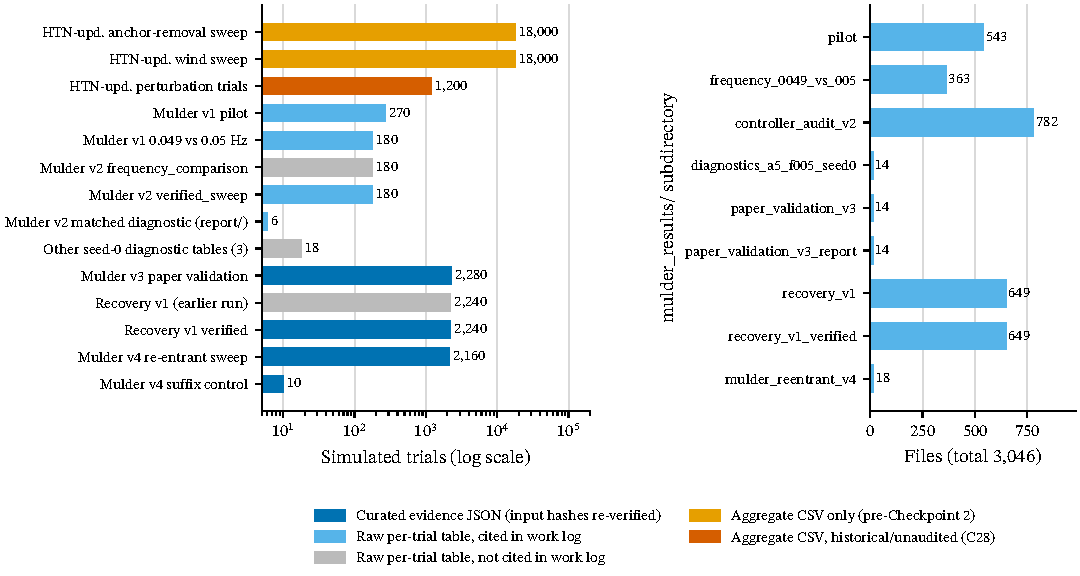
\includegraphics[width=\linewidth]{figures/record/record_evidence_volume}
  \caption{Evidence volume. \emph{Left:} simulated trials per study (log scale), coloured by how the result is held
  in the repository. Per-trial counts are data rows of each \texttt{trials.csv} under \texttt{mulder\_results/}
  (duplicate tables, e.g.\ \texttt{paper\_\allowbreak{}validation\_\allowbreak{}v3\_\allowbreak{}report}, are shown once), the suffix control is the
  \texttt{trials} list of \texttt{docs/\allowbreak{}research/\allowbreak{}evidence/\allowbreak{}mulder\_\allowbreak{}suffix\_\allowbreak{}control.json}, and the three
  \texttt{spider\_\allowbreak{}web\_\allowbreak{}htn\_\allowbreak{}updated} rows are the sums of the \texttt{n\_runs} column of
  \texttt{sensitivity\_\allowbreak{}comparison.csv}, \texttt{wind\_\allowbreak{}sensitivity.csv} and \texttt{perturbation\_\allowbreak{}trials.csv}.
  \emph{Right:} committed files per \texttt{mulder\_results/} subdirectory ($n=3{,}046$ files). Script
  \texttt{scripts/\allowbreak{}record/\allowbreak{}make\_\allowbreak{}figures.py}.}
  \label{fig:record-evidence}
\end{figure}

% --------------------------------------------------------------------------------------------
\subsection{Limitations and Next Steps}
\label{sec:record-limits}

We separate what has been done, what has been tested and found negative, and what has only been proposed.
Sources are the claim ledger, \texttt{MULDER\_\allowbreak{}OBJECTIVE\_\allowbreak{}ROADMAP.md}, the literature file and
\texttt{.ai-memory/\allowbreak{}ROADMAP.md}.

\paragraph{Done.}
\begin{itemize}
  \item A moving-support benchmark with six execution policies (C01), with a 2,280-trial paper-facing study (v3)
    in which ideal continuous local tracking completes 30/30 primary moving runs (C03) and endpoint execution
    fails (C02).
  \item A separate retained-tree recovery benchmark using unmodified IPyHOP, covering changed anchors,
    dependent suffixes, graph-valid detours and damaged prefixes within an authored sector domain (C16, C18--C20),
    with an explicitly backtracking fresh-planning baseline (C22).
  \item Retained-tree IPyHOP inside the actual Mulder HTN (v4, 2,160 trials; C24), with a ten-trial control.
  \item A planner-strategy audit correcting the project's description of backtracking (C15).
  \item The research record: work log, ledger, curated evidence with input hashes, snapshot, figure provenance,
    vendored and pinned dependencies; a targeted literature review with 14 bibliography entries.
\end{itemize}

\paragraph{Tested and negative.}
\begin{itemize}
  \item The HTN hierarchy gives no disturbance-tolerance advantage over the flat sequence in the Mulder benchmark:
    flat tracking matched the HTN's duration and outcomes on the tested phases (C06).
  \item Predictive repair does not beat local feedback (C07), and more frequent full replanning adds delay without
    improving completion (C08).
  \item Moving and stationary construction times are not identical in the model: local duration rises by about
    0.98\% with an interval excluding zero (C04).
  \item Results are not robust to sensory lag: 0/12 completion at 1\,s and 5\,s (C10).
  \item The \texttt{phase\_wait} alternative is slower, by 22.703291\,s on matched moving runs (C11).
  \item Mulder v3 recovery is fresh re-decomposition, not tree resumption (C13).
  \item Re-entrancy does not always reduce planning cost (C21); retained IPyHOP gives identical physical outcomes to
    fresh IPyHOP in all 720 Mulder pairs (C25); and fewer method calls did not mean faster planning (C26). The
    one scoped gain (C27) is reproduced by whole-suffix refresh without re-entrancy, and the small-size case regresses.
\end{itemize}

\paragraph{Not established.}
The simulator is not calibrated against the original cohort, whose raw observations have not been obtained (C12);
geometric invariance is largely imposed by prescribed counts and targets and cannot validate the biology (C09);
v3 does not handle arbitrary dependent suffixes or roadblocks (C14); historical runs do not guarantee backtracking
(C15); no joint quantitative conclusion across the packages is established, because the original HTN, updated HTN,
FAP and A* results still need a separate audit (C17); and the restored perturbation CSV does not demonstrate an HTN
advantage (C28). The comparative conclusion of Checkpoint~2's Section~9 therefore stands only as a description of
that specific random-walker comparison, not as a project-level finding. The team's own \texttt{insights.md} also
records that in the full anchor-removal sweep (\texttt{sensitivity\_\allowbreak{}comparison.csv}) the HTN's success rate falls to
0.822 at removal probability 0.8 while the baseline's is 0.999, because the baseline's completion check has no
structural-coherence requirement.

\paragraph{Proposed, not implemented.}
\begin{itemize}
  \item \emph{Objective roadmap milestones} (\texttt{MULDER\_\allowbreak{}OBJECTIVE\_\allowbreak{}ROADMAP.md}), all open: (1) a
    claim-to-measurement table marking every output as predicted, calibrated or imposed, with primary outcomes and
    agreement criteria fixed before tuning; (2) securing per-spider observations from the authors of
    Mulder et al.~\cite{mulder2021dynamic} (the article states they are available on reasonable request; no
    contact has been made); (3) fitting rigid controls only and freezing them; (4) testing moving-support
    predictions on effect sizes, accounting for repeated builds by the same spider; (5) testing the role of
    hierarchy under local rules, a flat sequence and HTN methods on the same movement model. Only the
    flat-sequence part of (5) exists (C06).
  \item \emph{E1, recovery determined by current web structure} (motivated by Peters and Eberhard): partial-web
    transfer kept distinct from damage, comparing history-only execution, a state-based rule controller, fresh-root
    HTN and retained HTN with shared observations and budgets. The literature file and \texttt{.ai-memory/\allowbreak{}ROADMAP.md}
    rank this first; it is backlog, not scheduled.
  \item \emph{E2, typical and atypical stage progression} (Corver, Zschokke): fixed-order vs.\ repeating-stage HTN
    vs.\ an equally informed finite-state model on held-out individuals, after the public data and licence are
    checked.
  \item \emph{E3, local geometry rules under task-level control} (Gotts, Krink and Vollrath, design variability):
    replace prescribed spiral waypoints with sensory rules and test geometry on held-out support shapes; the most
    substantial extension.
  \item \emph{Before any cross-package synthesis:} an independent audit of the original and updated HTN, FAP, A*
    and adaptive-planner code and outputs, including the historical perturbation study (C17, C28).
\end{itemize}
The literature file and project memory recommend a feasibility assessment and a fixed analysis protocol for E1 and
E2 before any implementation. More seeds would not help: as the roadmap puts it, more simulation cannot repair an
unvalidated physical assumption or create new animal observations.
